\documentclass[a4paper,12pt]{book} % The document class with options
\usepackage[T1]{fontenc}
\usepackage{lipsum} % Just for some filler text
\usepackage[margin=1in]{geometry}
\usepackage{xcolor}
\usepackage{graphicx}
\usepackage{array}
\usepackage{booktabs}
\usepackage{amsmath}
\usepackage[parfill]{parskip}
%\usepackage{natbib}
\usepackage[style=authoryear]{biblatex}
\addbibresource{first.bib} 
\newcommand\kw[1]{\textcolor{red}{\itshape #1}}
\usepackage{fontspec}
\setmainfont{texgyretermes-regular.otf}
\newfontfamily\cjkfont{FandolSong-Regular.otf}
\usepackage{mhchem}
\usepackage{forest}
\usepackage{xskak}
\usepackage{tikz}
\usepackage{pgfplots}
%\usepackage{musixtex}
\pgfplotsset{width=7cm,compat=1.16}
\usetikzlibrary {perspective}
% A comment in the preamble
% \newcommand\kw[1]{\textbf{\itshape #1}}

\begin{document}

%
\documentclass[a4paper,12pt]{book} % The document class with options

	\usepackage{musixtex}
\begin{document}

\begin{center}
\begin{music}
	\parindent10mm
	\instrumentnumber{1}
	% a single instrument
	\setname1{Piano}
	% whose name is Piano
	\setstaffs1{2}
	% with two staffs
	\generalmeter{\meterfrac44}
	% 4/4 meter chosen
	\startextract
	% starting real score
	\Notes\ibu0f0\qb0{cge}\tbu0\qb0g|\hl j\en
	\Notes\ibu0f0\qb0{cge}\tbu0\qb0g|\ql l\sk\ql n\en
	\bar
	\Notes\ibu0f0\qb0{dgf}|\qlp i\en
	\notes\tbu0\qb0g|\ibbl1j3\qb1j\tbl1\qb1k\en
	\Notes\ibu0f0\qb0{cge}\tbu0\qb0g|\hl j\en
	\zendextract
	% terminate excerpt
\end{music}
\end{center}

\end{document}


% This is a comment
This is~~~~~\textbf{a}~~~~~simple
document\footnote{with a footnote}.

This is a new paragraph.

Some text with \emph{emphasis and \emph{nested} content}.

Some text in \textit{italic and \textbf{nested} content}.

Hey world!
\lipsum
This is a first document.

\section{Title of the first section}

Text of material in the first section

Second paragraph.

\subsection{Subsection of the first section}

\newchessgame
\mainline{1. e4 e5 2. Nf3 Nc6 3. Bb5 a6 4. Ba4 Nf6}

\xskakset{moveid=2w}%
\chessboard[setfen=\xskakget{nextfen}]\\[1ex]
Position after 2.\,\xskakget{lan}

\chapter{1}
Text of material in the subsection.

\begin{forest}
  [VP
    [DP[John]]
    [V’
      [V[sent]]
      [DP[Mary]]
      [DP[D[a]][NP[letter]]]
    ]
  ]
\end{forest}

\newcommand\simplecuboid[3]{%
  \fill[gray!80!white] (tpp cs:x=0,y=0,z=#3)
  -- (tpp cs:x=0,y=#2,z=#3)
  -- (tpp cs:x=#1,y=#2,z=#3)
  -- (tpp cs:x=#1,y=0,z=#3) -- cycle;
  x
  \fill[gray] (tpp cs:x=0,y=0,z=0)
  -- (tpp cs:x=0,y=0,z=#3)
  -- (tpp cs:x=0,y=#2,z=#3)
  -- (tpp cs:x=0,y=#2,z=0) -- cycle;
  \fill[gray!50!white] (tpp cs:x=0,y=0,z=0)
  -- (tpp cs:x=0,y=0,z=#3)
  -- (tpp cs:x=#1,y=0,z=#3)
  -- (tpp cs:x=#1,y=0,z=0) -- cycle;}
\newcommand{\simpleaxes}[3]{%
  \draw[->] (-0.5,0,0) -- (#1,0,0) node[pos=1.1]{x};
  \draw[->] (0,-0.5,0) -- (0,#2,0) node[pos=1.1]{y};
  \draw[->] (0,0,-0.5) -- (0,0,#3) node[pos=1.1]{z};}
\begin{tikzpicture}[3d view]
  \simplecuboid{2}{2}{2}
  \simpleaxes{2}{2}{2}
\end{tikzpicture}

\section{Second section}
Text of the second section.
\\
Ordered
\begin{enumerate}
\item An entry
\item Another One
\item Wow! Three entries
\end{enumerate}

Unordered
\begin{itemize}
\item An entry
\item Another One
\item Wow! Three entries
\end{itemize}

Something about \kw{apples} and \kw{oranges}.
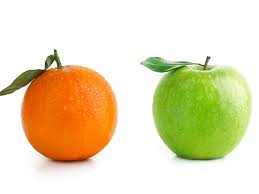
\includegraphics[height=4cm]{first.jpeg}
\begin{center}
  \begin{figure}[ht]
    \centering
    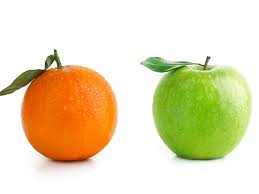
\includegraphics[height=4cm,clip, trim = 5 5 5 5]{first.jpeg}
    \caption{An example image}
  \end{figure}
\end{center}
\begin{tabular}{lll}
  Animal & Food  & Size   \\
  dog    & meat  & medium \\
  horse  & hay   & large  \\
  frog   & flies & small  \\
\end{tabular}

\begin{tabular}{lll}
  Animal & Description \\
  dog    & The dog is a member of the genus Canis, which forms part of the
  wolf-like canids, and is the most widely abundant terrestrial
  carnivore. \\
  cat    & The cat is a domestic species of small carnivorous mammal. It is the
  \\
  only domesticated species in the family Felidae and is often referred
  \\   
  to as the domestic cat to distinguish it from the wild members of the
  \\ 
  family. \\
\end{tabular}

\begin{tabular}{lll}
  \toprule
  Animal & Food  & Size   \\
  \midrule
  dog    & meat  & medium \\
  \cmidrule{1-2}
  horse  & hay   & large  \\
  \cmidrule{1-1}
  \cmidrule{3-3}
  frog   & flies & small  \\
  \bottomrule
\end{tabular}

\begin{tabular}{lll}
  \toprule
  Group     & Animal & Size   \\
  \midrule
  herbivore & horse  & large  \\
  & deer   & medium \\
  & rabbit & small  \\
  \addlinespace
  carnivore & dog    & medium \\
  & cat    & small  \\
  & lion   & large  \\
  \addlinespace
  omnivore  & crow   & small  \\
  & bear   & large  \\
  & pig    & medium \\
  \bottomrule
\end{tabular}

Text of material for the first subsection.
\begin{equation}
  e^{i\pi}+1 = 0
  \label{eq:labeltwo}
\end{equation}

\begin{equation}
  \int_{-\infty}^{+\infty} e^{-x^2} \, dx
\end{equation}

Solve the following recurrence for $ n,k\geq 0 $:
\begin{align*}
  Q_{n,0} &= 1   \quad Q_{0,k} = [k=0];  \\
  Q_{n,k} &= Q_{n-1,k}+Q_{n-1,k-1}+\binom{n}{k}, \quad\text{for $n$, $k>0$.}
\end{align*}

AMS matrices.
\[
\begin{matrix}
  a & b & c \\
  d & e & f
\end{matrix}
\quad
\begin{pmatrix}
  a & b & c \\
  d & e & f
\end{pmatrix}
\quad
\begin{bmatrix}
  a & b & c \\
  d & e & f
\end{bmatrix}
\]

\ce{Hg^2+ ->[I-] HgI2 ->[I-] [Hg^{II}I4]^2-}

ABC → αβγ → {\cjkfont 你好}

$\text{bad use } size  \neq \mathit{size} \neq \mathrm{size} $

\textit{$\text{bad use } size \neq \mathit{size} \neq \mathrm{size} $}

Some text \hspace{1cm} more text.

\vspace{10cm}

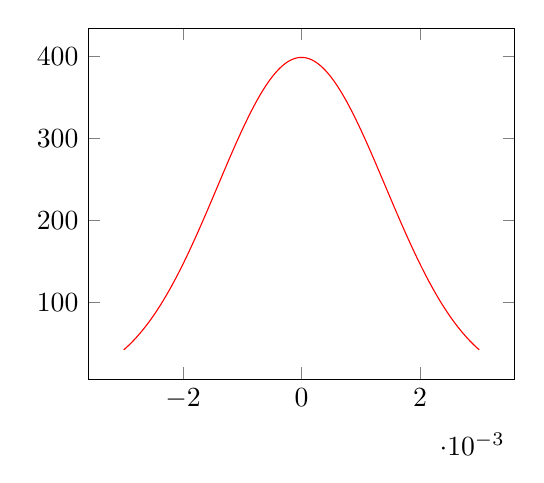
\begin{tikzpicture}
  \begin{axis}[]
    % density of Normal distribution:
    \addplot [
      red,
      domain=-3e-3:3e-3,
      samples=201,
    ]
             {exp(-x^2 / (2e-3^2)) / (1e-3 * sqrt(2*pi))};
  \end{axis}
\end{tikzpicture}

The mathematics showcase is from \autocite{Graham1995}.

Some more complex citations: \parencite{Graham1995} or
\textcite{Thomas2008} or possibly \citetitle{Graham1995}.

\autocite[56]{Thomas2008}

\autocite[See][45-48]{Graham1995}

Together \autocite{Thomas2008,Graham1995}

\printbibliography

\end{document}
